\documentclass[12pt,a4paper]{article}
\usepackage[utf8]{vietnam}
\usepackage{amsmath,amssymb}
\usepackage{tabularx}
\usepackage{tikz}
\usepackage{xcolor}
\usepackage[top=0.6cm, bottom=0.6cm, left=0.6cm, right=0.6cm]{geometry}
\usepackage[dethi]{ex_test}

\setlength{\parskip}{0pt}

% Dòng kẻ chấm mờ đều đặn chuẩn viết tay (khoảng cách 7.2mm rộng rãi)
\newcommand{\dongke}[1]{%
  \begingroup%
  \setlength{\parskip}{0pt}%
  \baselineskip=20.5pt%
  \vspace{1.5mm}%
  \foreach \i in {1,...,#1}{%
    \noindent{\color{gray!60}\dotfill}\par%
  }%
  \vspace{1mm}%
  \endgroup%
}

% Định nghĩa ô bài tập tự luận trong bảng
\newcommand{\oBaiTap}[3][6]{%
  \vspace{1.5mm}%
  \noindent\textbf{#2} #3\par%
  \dongke{#1}%
}

% Câu trắc nghiệm 1 cột: 4 đáp án dàn hàng ngang trên 1 dòng
\newcommand{\cauTN}[6]{% \cauTN{số câu}{đề}{A}{B}{C}{D}
  \noindent\textbf{Câu #1.} #2\par\vspace{0.4mm}%
  \noindent%
  \makebox[0.25\linewidth][l]{\textbf{A.} #3}%
  \makebox[0.25\linewidth][l]{\textbf{B.} #4}%
  \makebox[0.25\linewidth][l]{\textbf{C.} #5}%
  \makebox[0.25\linewidth][l]{\textbf{D.} #6}\par\vspace{0.8mm}%
}

\begin{document}
\pagestyle{empty}
% =============================================================================
% ========================= TOÁN 7 - TUẦN 05 - BUỔI 01: MÃ ĐỀ 101 =============
% ========================= MẶT TRƯỚC (TRANG 1/2) ==============================
% =============================================================================

\noindent
\begin{tabularx}{\linewidth}{|X|c|}
\hline
\textbf{PHIẾU KIỂM TRA ĐỊNH KỲ TOÁN 7 - TUẦN 05 - BUỔI 01} & \textbf{Mã đề: 101 - Trang 1/2} \\
\textit{Chủ đề: Bài 7: Tập hợp các số thực. Giá trị tuyệt đối của một số thực} & \textit{Thời gian: 45 phút} \\
\hline
\end{tabularx}

\vspace{1mm}

\noindent
\begin{tabularx}{\linewidth}{|X|}
\hline
\rule[-2.5mm]{0pt}{8.5mm}\textbf{Họ và tên học sinh:} \hfill \textbf{SĐT:} \makebox[4.5cm]{\dotfill} \\
\hline
\end{tabularx}

\vspace{1mm}

\noindent
\begin{tabularx}{\linewidth}{|p{3.2cm}|X|}
\hline
\centering\textbf{ĐIỂM SỐ} & \centering\textbf{LỜI NHẬN XÉT CỦA THẦY CÔ} \tabularnewline
\hline
\rule{0pt}{1.8cm} & \tabularnewline
\hline
\end{tabularx}

\vspace{1.5mm}

\noindent\textbf{\large PHẦN I. TRẮC NGHIỆM KHÁCH QUAN (2,5 điểm)} \hfill \textit{(Khoanh tròn đáp án đúng)}
\vspace{1mm}

\cauTN{1}{Khẳng định nào sau đây là \textbf{sai}?}{$\mathbb{N} \subset \mathbb{Z}$}{$\mathbb{Z} \subset \mathbb{Q}$}{$\mathbb{Q} \subset \mathbb{R}$}{$\mathbb{I} \subset \mathbb{Q}$}

\cauTN{2}{Số đối của số thực $-\sqrt{7}$ là:}{$\sqrt{7}$}{$-\sqrt{7}$}{$7$}{$-7$}

\cauTN{3}{Giá trị của biểu thức $|-3{,}45|$ là:}{$-3{,}45$}{$3{,}45$}{$\pm 3{,}45$}{$0$}

\cauTN{4}{Khẳng định nào sau đây là \textbf{đúng}?}{$-2{,}5 > -2{,}4$}{$\sqrt{3} < 1{,}7$}{$\sqrt{5} > 2$}{$-\pi > 0$}

\cauTN{5}{Cho đường thẳng $c$ cắt hai đường thẳng $a$ và $b$. Nếu $a \parallel b$ thì hai góc so le trong:}{bù nhau}{phụ nhau}{bằng nhau}{có tổng bằng $90^\circ$}

\vspace{1.2mm}

\noindent\textbf{\large PHẦN II. TỰ LUẬN (7,5 điểm)}

\noindent\textbf{Câu 2 (2,5 điểm). Thực hiện phép tính (hợp lý nếu có thể):}
\vspace{0.8mm}

\noindent
\begin{tabularx}{\linewidth}{|X|X|}
\hline
\oBaiTap[7]{a)}{$\sqrt{\dfrac{16}{25}} - |-0{,}8| + \dfrac{3}{4}$} & 
\oBaiTap[7]{b)}{$\dfrac{13}{17} \cdot |-2{,}4| + \dfrac{4}{17} \cdot 2{,}4$} \\
\hline
\oBaiTap[7]{c)}{$\left(-\dfrac{1}{2}\right)^2 + \sqrt{0{,}09} - \left|\dfrac{5}{4} - 1\right|$} & 
\oBaiTap[7]{d)}{$\dfrac{5}{6} : \left[\dfrac{2}{3} - \left(0{,}75 - \left|-\dfrac{1}{2}\right|\right)\right]$} \\
\hline
\end{tabularx}

\newpage
% =============================================================================
% ========================= TOÁN 7 - TUẦN 05 - BUỔI 01: MÃ ĐỀ 101 =============
% ========================= MẶT SAU (TRANG 2/2) ================================
% =============================================================================

\noindent
\begin{tabularx}{\linewidth}{|X|c|}
\hline
\textbf{PHẦN II. TỰ LUẬN (Tiếp theo) - TOÁN 7 TUẦN 05 BUỔI 01} & \textbf{Mã đề: 101 - Trang 2/2} \\
\hline
\end{tabularx}


\vspace{2mm}

\noindent\textbf{\large Câu 3 (2,5 điểm). Tìm số thực $x$, biết:}
\vspace{0.8mm}

\noindent
\begin{tabularx}{\linewidth}{|X|X|}
\hline
\oBaiTap[6]{a)}{$|x| - \dfrac{3}{4} = \dfrac{1}{2}$} & 
\oBaiTap[6]{b)}{$\left|x - \dfrac{1}{2}\right| = \dfrac{3}{4}$} \\
\hline
\oBaiTap[6]{c)}{$2\left|x + \dfrac{1}{3}\right| - \dfrac{1}{2} = \dfrac{5}{6}$} & 
\oBaiTap[6]{d)}{$\left|2x - \dfrac{1}{5}\right| = \dfrac{4}{5}$} \\
\hline
\end{tabularx}

\vspace{2mm}

\noindent\textbf{\large Câu 4 (2,5 điểm).} Cho hình vẽ, biết $a \parallel b$:\par\vspace{0.6mm}
\noindent\textbf{a) (1,25 điểm)} Tính số đo góc $\widehat{A}_2$ và góc $\widehat{A}_3$.\par\vspace{0.4mm}
\noindent\textbf{b) (1,25 điểm)} Tính số đo góc $\widehat{B}_3$ và góc $\widehat{B}_1$.\par\vspace{1mm}

\noindent
\begin{tabularx}{\linewidth}{|p{5.5cm}|X|}
\hline
\vspace{1.5mm}
\centering
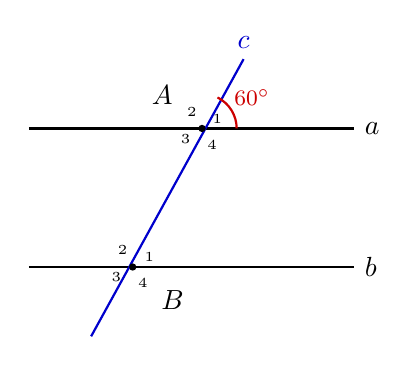
\begin{tikzpicture}[>=stealth, scale=0.88]
    \draw[thick] (-1.5, 2) -- (3.2, 2) node[right] {$a$};
    \draw[thick] (-1.5, 0) -- (3.2, 0) node[right] {$b$};
    \draw[thick, blue!80!black] (-0.6, -1.0) -- (1.6, 3.0) node[above] {$c$};
    
    \coordinate (A) at (1, 2);
    \coordinate (B) at (0, 0);
    
    \fill (A) circle (1.5pt);
    \fill (B) circle (1.5pt);
    
    \path (A) ++(140:0.75) node[font=\bfseries] {$A$};
    \path (B) ++(320:0.75) node[font=\bfseries] {$B$};
    
    \draw[red!80!black, thick] (A) ++(0:0.5) arc (0:63.4:0.5);
    \path (A) ++(31.7:0.85) node[red!80!black, font=\footnotesize] {$60^\circ$};
    
    \path (A) ++(31.7:0.26) node[font=\tiny] {$1$};
    \path (A) ++(121.7:0.28) node[font=\tiny] {$2$};
    \path (A) ++(211.7:0.28) node[font=\tiny] {$3$};
    \path (A) ++(301.7:0.28) node[font=\tiny] {$4$};
    
    \path (B) ++(31.7:0.28) node[font=\tiny] {$1$};
    \path (B) ++(121.7:0.28) node[font=\tiny] {$2$};
    \path (B) ++(211.7:0.28) node[font=\tiny] {$3$};
    \path (B) ++(301.7:0.28) node[font=\tiny] {$4$};
\end{tikzpicture}
\vspace{1.5mm}
&
\vspace{0.8mm}
\noindent\textit{Bài giải:}\par
\dongke{17}
\\ \hline
\end{tabularx}

\newpage
% =============================================================================
% ========================= TOÁN 7 - TUẦN 05 - BUỔI 01: MÃ ĐỀ 102 =============
% ========================= MẶT TRƯỚC (TRANG 1/2) ==============================
% =============================================================================

\noindent
\begin{tabularx}{\linewidth}{|X|c|}
\hline
\textbf{PHIẾU KIỂM TRA ĐỊNH KỲ TOÁN 7 - TUẦN 05 - BUỔI 01} & \textbf{Mã đề: 102 - Trang 1/2} \\
\textit{Chủ đề: Bài 7: Tập hợp các số thực. Giá trị tuyệt đối của một số thực} & \textit{Thời gian: 45 phút} \\
\hline
\end{tabularx}

\vspace{1mm}

\noindent
\begin{tabularx}{\linewidth}{|X|}
\hline
\rule[-2.5mm]{0pt}{8.5mm}\textbf{Họ và tên học sinh:} \hfill \textbf{SĐT:} \makebox[4.5cm]{\dotfill} \\
\hline
\end{tabularx}

\vspace{1mm}

\noindent
\begin{tabularx}{\linewidth}{|p{3.2cm}|X|}
\hline
\centering\textbf{ĐIỂM SỐ} & \centering\textbf{LỜI NHẬN XÉT CỦA THẦY CÔ} \tabularnewline
\hline
\rule{0pt}{1.8cm} & \tabularnewline
\hline
\end{tabularx}

\vspace{1.5mm}

\noindent\textbf{\large PHẦN I. TRẮC NGHIỆM KHÁCH QUAN (2,5 điểm)} \hfill \textit{(Khoanh tròn đáp án đúng)}
\vspace{1mm}

\cauTN{1}{Khẳng định nào sau đây là \textbf{đúng}?}{$\sqrt{2} \in \mathbb{Q}$}{$\mathbb{Q} \cup \mathbb{I} = \mathbb{R}$}{$\mathbb{R} \subset \mathbb{Q}$}{$-5 \in \mathbb{N}$}

\cauTN{2}{Số đối của số thực $\pi$ là:}{$\pi$}{$-\pi$}{$3{,}14$}{$-3{,}14$}

\cauTN{3}{Giá trị của biểu thức $|1 - \sqrt{2}|$ bằng:}{$1 - \sqrt{2}$}{$\sqrt{2} - 1$}{$\sqrt{2} + 1$}{$-1 - \sqrt{2}$}

\cauTN{4}{Trong các số thực sau, số nào nhỏ nhất?}{$-1{,}5$}{$-\sqrt{3}$}{$0$}{$1$}

\cauTN{5}{Cho hai đường thẳng song song $a \parallel b$ bị cắt bởi đường thẳng $c$. Hai góc đồng vị thì:}{bù nhau}{bằng nhau}{kề nhau}{kề bù}

\vspace{1.2mm}

\noindent\textbf{\large PHẦN II. TỰ LUẬN (7,5 điểm)}

\noindent\textbf{Câu 2 (2,5 điểm). Thực hiện phép tính (hợp lý nếu có thể):}
\vspace{0.8mm}

\noindent
\begin{tabularx}{\linewidth}{|X|X|}
\hline
\oBaiTap[7]{a)}{$\sqrt{\dfrac{9}{16}} - |-0{,}75| + \dfrac{2}{5}$} & 
\oBaiTap[7]{b)}{$\dfrac{11}{15} \cdot |-3{,}6| + \dfrac{4}{15} \cdot 3{,}6$} \\
\hline
\oBaiTap[7]{c)}{$\left(-\dfrac{1}{2}\right)^2 + \sqrt{0{,}16} - \left|\dfrac{3}{4} - \dfrac{1}{2}\right|$} & 
\oBaiTap[7]{d)}{$\dfrac{7}{12} : \left[\dfrac{3}{4} - \left(0{,}5 - \left|-\dfrac{1}{3}\right|\right)\right]$} \\
\hline
\end{tabularx}

\newpage
% =============================================================================
% ========================= TOÁN 7 - TUẦN 05 - BUỔI 01: MÃ ĐỀ 102 =============
% ========================= MẶT SAU (TRANG 2/2) ================================
% =============================================================================

\noindent
\begin{tabularx}{\linewidth}{|X|c|}
\hline
\textbf{PHẦN II. TỰ LUẬN (Tiếp theo) - TOÁN 7 TUẦN 05 BUỔI 01} & \textbf{Mã đề: 102 - Trang 2/2} \\
\hline
\end{tabularx}


\vspace{2mm}

\noindent\textbf{\large Câu 3 (2,5 điểm). Tìm số thực $x$, biết:}
\vspace{0.8mm}

\noindent
\begin{tabularx}{\linewidth}{|X|X|}
\hline
\oBaiTap[6]{a)}{$|x| - \dfrac{2}{3} = \dfrac{1}{6}$} & 
\oBaiTap[6]{b)}{$\left|x - \dfrac{1}{3}\right| = \dfrac{2}{3}$} \\
\hline
\oBaiTap[6]{c)}{$3\left|x + \dfrac{1}{4}\right| - \dfrac{1}{2} = 1$} & 
\oBaiTap[6]{d)}{$\left|2x - \dfrac{1}{3}\right| = \dfrac{5}{3}$} \\
\hline
\end{tabularx}

\vspace{2mm}

\noindent\textbf{\large Câu 4 (2,5 điểm).} Cho hình vẽ, biết $a \parallel b$:\par\vspace{0.6mm}
\noindent\textbf{a) (1,25 điểm)} Tính số đo góc $\widehat{A}_1$ và góc $\widehat{A}_4$.\par\vspace{0.4mm}
\noindent\textbf{b) (1,25 điểm)} Tính số đo góc $\widehat{B}_4$ và góc $\widehat{B}_2$.\par\vspace{1mm}

\noindent
\begin{tabularx}{\linewidth}{|p{5.5cm}|X|}
\hline
\vspace{1.5mm}
\centering
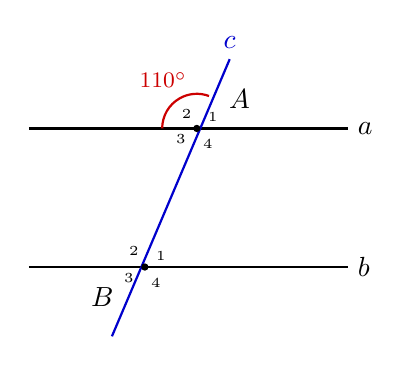
\begin{tikzpicture}[>=stealth, scale=0.88]
    \draw[thick] (-1.8, 2) -- (2.8, 2) node[right] {$a$};
    \draw[thick] (-1.8, 0) -- (2.8, 0) node[right] {$b$};
    \draw[thick, blue!80!black] (-0.6, -1.0) -- (1.1, 3.0) node[above] {$c$};
    
    \coordinate (A) at (0.625, 2);
    \coordinate (B) at (-0.125, 0);
    
    \fill (A) circle (1.5pt);
    \fill (B) circle (1.5pt);
    
    \path (A) ++(35:0.75) node[font=\bfseries] {$A$};
    \path (B) ++(215:0.75) node[font=\bfseries] {$B$};
    
    \draw[red!80!black, thick] (A) ++(180:0.5) arc (180:69.4:0.5);
    \path (A) ++(124.7:0.85) node[red!80!black, font=\footnotesize] {$110^\circ$};
    
    \path (A) ++(34.7:0.28) node[font=\tiny] {$1$};
    \path (A) ++(124.7:0.26) node[font=\tiny] {$2$};
    \path (A) ++(214.7:0.28) node[font=\tiny] {$3$};
    \path (A) ++(304.7:0.28) node[font=\tiny] {$4$};
    
    \path (B) ++(34.7:0.28) node[font=\tiny] {$1$};
    \path (B) ++(124.7:0.28) node[font=\tiny] {$2$};
    \path (B) ++(214.7:0.28) node[font=\tiny] {$3$};
    \path (B) ++(304.7:0.28) node[font=\tiny] {$4$};
\end{tikzpicture}
\vspace{1.5mm}
&
\vspace{0.8mm}
\noindent\textit{Bài giải:}\par
\dongke{17}
\\ \hline
\end{tabularx}

\newpage
% =============================================================================
% ========================= TOÁN 7 - TUẦN 05 - BUỔI 01: MÃ ĐỀ 103 =============
% ========================= MẶT TRƯỚC (TRANG 1/2) ==============================
% =============================================================================

\noindent
\begin{tabularx}{\linewidth}{|X|c|}
\hline
\textbf{PHIẾU KIỂM TRA ĐỊNH KỲ TOÁN 7 - TUẦN 05 - BUỔI 01} & \textbf{Mã đề: 103 - Trang 1/2} \\
\textit{Chủ đề: Bài 7: Tập hợp các số thực. Giá trị tuyệt đối của một số thực} & \textit{Thời gian: 45 phút} \\
\hline
\end{tabularx}

\vspace{1mm}

\noindent
\begin{tabularx}{\linewidth}{|X|}
\hline
\rule[-2.5mm]{0pt}{8.5mm}\textbf{Họ và tên học sinh:} \hfill \textbf{SĐT:} \makebox[4.5cm]{\dotfill} \\
\hline
\end{tabularx}

\vspace{1mm}

\noindent
\begin{tabularx}{\linewidth}{|p{3.2cm}|X|}
\hline
\centering\textbf{ĐIỂM SỐ} & \centering\textbf{LỜI NHẬN XÉT CỦA THẦY CÔ} \tabularnewline
\hline
\rule{0pt}{1.8cm} & \tabularnewline
\hline
\end{tabularx}

\vspace{1.5mm}

\noindent\textbf{\large PHẦN I. TRẮC NGHIỆM KHÁCH QUAN (2,5 điểm)} \hfill \textit{(Khoanh tròn đáp án đúng)}
\vspace{1mm}

\cauTN{1}{Tập hợp các số thực được ký hiệu là:}{$\mathbb{Q}$}{$\mathbb{Z}$}{$\mathbb{R}$}{$\mathbb{I}$}

\cauTN{2}{Số đối của số thực $2{,}5$ là:}{$2{,}5$}{$\dfrac{5}{2}$}{$-2{,}5$}{$\dfrac{2}{5}$}

\cauTN{3}{Khẳng định nào sau đây đúng với mọi số thực $x$?}{$|x| < 0$}{$|x| \le 0$}{$|x| \ge 0$}{$|x| > 0$}

\cauTN{4}{So sánh hai số thực $x = \sqrt{10}$ và $y = 3$:}{$x < y$}{$x > y$}{$x = y$}{$x \le y$}

\cauTN{5}{Hai góc trong cùng phía tạo bởi một đường thẳng cắt hai đường thẳng song song thì:}{bằng nhau}{phụ nhau}{bù nhau}{đối đỉnh}

\vspace{1.2mm}

\noindent\textbf{\large PHẦN II. TỰ LUẬN (7,5 điểm)}

\noindent\textbf{Câu 2 (2,5 điểm). Thực hiện phép tính (hợp lý nếu có thể):}
\vspace{0.8mm}

\noindent
\begin{tabularx}{\linewidth}{|X|X|}
\hline
\oBaiTap[7]{a)}{$\sqrt{\dfrac{49}{100}} - |-0{,}7| + \dfrac{3}{5}$} & 
\oBaiTap[7]{b)}{$\dfrac{7}{19} \cdot |-4{,}5| + \dfrac{12}{19} \cdot 4{,}5$} \\
\hline
\oBaiTap[7]{c)}{$\left(-\dfrac{1}{2}\right)^2 + \sqrt{0{,}25} - \left|\dfrac{7}{4} - 1{,}5\right|$} & 
\oBaiTap[7]{d)}{$\dfrac{3}{4} : \left[\dfrac{5}{6} - \left(0{,}8 - \left|-\dfrac{3}{10}\right|\right)\right]$} \\
\hline
\end{tabularx}

\newpage
% =============================================================================
% ========================= TOÁN 7 - TUẦN 05 - BUỔI 01: MÃ ĐỀ 103 =============
% ========================= MẶT SAU (TRANG 2/2) ================================
% =============================================================================

\noindent
\begin{tabularx}{\linewidth}{|X|c|}
\hline
\textbf{PHẦN II. TỰ LUẬN (Tiếp theo) - TOÁN 7 TUẦN 05 BUỔI 01} & \textbf{Mã đề: 103 - Trang 2/2} \\
\hline
\end{tabularx}


\vspace{2mm}

\noindent\textbf{\large Câu 3 (2,5 điểm). Tìm số thực $x$, biết:}
\vspace{0.8mm}

\noindent
\begin{tabularx}{\linewidth}{|X|X|}
\hline
\oBaiTap[6]{a)}{$|x| - \dfrac{1}{2} = \dfrac{2}{5}$} & 
\oBaiTap[6]{b)}{$\left|x - \dfrac{2}{5}\right| = \dfrac{3}{5}$} \\
\hline
\oBaiTap[6]{c)}{$2\left|x + \dfrac{1}{2}\right| - \dfrac{3}{4} = \dfrac{3}{4}$} & 
\oBaiTap[6]{d)}{$\left|2x - \dfrac{1}{4}\right| = \dfrac{7}{4}$} \\
\hline
\end{tabularx}

\vspace{2mm}

\noindent\textbf{\large Câu 4 (2,5 điểm).} Cho hình vẽ, biết $a \parallel b$:\par\vspace{0.6mm}
\noindent\textbf{a) (1,25 điểm)} Tính số đo góc $\widehat{A}_4$ và góc $\widehat{A}_1$.\par\vspace{0.4mm}
\noindent\textbf{b) (1,25 điểm)} Tính số đo góc $\widehat{B}_1$ và góc $\widehat{B}_3$.\par\vspace{1mm}

\noindent
\begin{tabularx}{\linewidth}{|p{5.5cm}|X|}
\hline
\vspace{1.5mm}
\centering
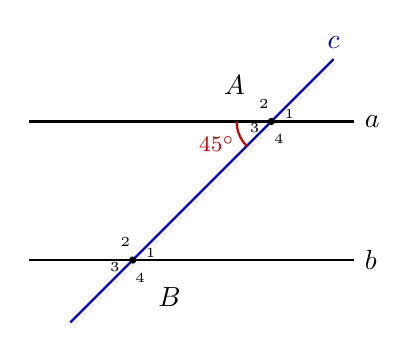
\begin{tikzpicture}[>=stealth, scale=0.88]
    \draw[thick] (-1.5, 2) -- (3.2, 2) node[right] {$a$};
    \draw[thick] (-1.5, 0) -- (3.2, 0) node[right] {$b$};
    \draw[thick, blue!80!black] (-0.9, -0.9) -- (2.9, 2.9) node[above] {$c$};
    
    \coordinate (A) at (2, 2);
    \coordinate (B) at (0, 0);
    
    \fill (A) circle (1.5pt);
    \fill (B) circle (1.5pt);
    
    \path (A) ++(135:0.75) node[font=\bfseries] {$A$};
    \path (B) ++(315:0.75) node[font=\bfseries] {$B$};
    
    \draw[red!80!black, thick] (A) ++(180:0.5) arc (180:225:0.5);
    \path (A) ++(202.5:0.85) node[red!80!black, font=\footnotesize] {$45^\circ$};
    
    \path (A) ++(22.5:0.28) node[font=\tiny] {$1$};
    \path (A) ++(112.5:0.28) node[font=\tiny] {$2$};
    \path (A) ++(202.5:0.26) node[font=\tiny] {$3$};
    \path (A) ++(292.5:0.28) node[font=\tiny] {$4$};
    
    \path (B) ++(22.5:0.28) node[font=\tiny] {$1$};
    \path (B) ++(112.5:0.28) node[font=\tiny] {$2$};
    \path (B) ++(202.5:0.28) node[font=\tiny] {$3$};
    \path (B) ++(292.5:0.28) node[font=\tiny] {$4$};
\end{tikzpicture}
\vspace{1.5mm}
&
\vspace{0.8mm}
\noindent\textit{Bài giải:}\par
\dongke{17}
\\ \hline
\end{tabularx}

\newpage
% =============================================================================
% ========================= TOÁN 7 - TUẦN 05 - BUỔI 01: MÃ ĐỀ 104 =============
% ========================= MẶT TRƯỚC (TRANG 1/2) ==============================
% =============================================================================

\noindent
\begin{tabularx}{\linewidth}{|X|c|}
\hline
\textbf{PHIẾU KIỂM TRA ĐỊNH KỲ TOÁN 7 - TUẦN 05 - BUỔI 01} & \textbf{Mã đề: 104 - Trang 1/2} \\
\textit{Chủ đề: Bài 7: Tập hợp các số thực. Giá trị tuyệt đối của một số thực} & \textit{Thời gian: 45 phút} \\
\hline
\end{tabularx}

\vspace{1mm}

\noindent
\begin{tabularx}{\linewidth}{|X|}
\hline
\rule[-2.5mm]{0pt}{8.5mm}\textbf{Họ và tên học sinh:} \hfill \textbf{SĐT:} \makebox[4.5cm]{\dotfill} \\
\hline
\end{tabularx}

\vspace{1mm}

\noindent
\begin{tabularx}{\linewidth}{|p{3.2cm}|X|}
\hline
\centering\textbf{ĐIỂM SỐ} & \centering\textbf{LỜI NHẬN XÉT CỦA THẦY CÔ} \tabularnewline
\hline
\rule{0pt}{1.8cm} & \tabularnewline
\hline
\end{tabularx}

\vspace{1.5mm}

\noindent\textbf{\large PHẦN I. TRẮC NGHIỆM KHÁCH QUAN (2,5 điểm)} \hfill \textit{(Khoanh tròn đáp án đúng)}
\vspace{1mm}

\cauTN{1}{Chọn khẳng định \textbf{đúng}:}{$\pi \in \mathbb{Q}$}{$\sqrt{5} \in \mathbb{R}$}{$-\dfrac{3}{4} \in \mathbb{I}$}{$0 \in \mathbb{I}$}

\cauTN{2}{Số đối của số thực $-\dfrac{\sqrt{3}}{2}$ là:}{$\dfrac{\sqrt{3}}{2}$}{$-\dfrac{\sqrt{3}}{2}$}{$\dfrac{3}{2}$}{$-\dfrac{3}{2}$}

\cauTN{3}{Giá trị của biểu thức $|-\sqrt{9}|$ là:}{$-3$}{$3$}{$9$}{$-9$}

\cauTN{4}{Khẳng định nào sau đây là \textbf{sai}?}{$0 > -1{,}2$}{$\sqrt{4} = 2$}{$-1{,}5 > -\sqrt{2}$}{$1{,}41 < \sqrt{2}$}

\cauTN{5}{Nếu một đường thẳng cắt hai đường thẳng song song thì:}{Hai góc đồng vị bù nhau}{Hai góc so le trong bằng nhau}{Hai góc so le trong bù nhau}{Hai góc kề bù bằng nhau}

\vspace{1.2mm}

\noindent\textbf{\large PHẦN II. TỰ LUẬN (7,5 điểm)}

\noindent\textbf{Câu 2 (2,5 điểm). Thực hiện phép tính (hợp lý nếu có thể):}
\vspace{0.8mm}

\noindent
\begin{tabularx}{\linewidth}{|X|X|}
\hline
\oBaiTap[7]{a)}{$\sqrt{\dfrac{36}{25}} - |-1{,}2| + \dfrac{4}{5}$} & 
\oBaiTap[7]{b)}{$\dfrac{9}{23} \cdot |-5{,}2| + \dfrac{14}{23} \cdot 5{,}2$} \\
\hline
\oBaiTap[7]{c)}{$\left(-\dfrac{1}{2}\right)^2 + \sqrt{0{,}36} - \left|\dfrac{5}{4} - 1\right|$} & 
\oBaiTap[7]{d)}{$\dfrac{2}{3} : \left[\dfrac{4}{5} - \left(0{,}6 - \left|-\dfrac{1}{4}\right|\right)\right]$} \\
\hline
\end{tabularx}

\newpage
% =============================================================================
% ========================= TOÁN 7 - TUẦN 05 - BUỔI 01: MÃ ĐỀ 104 =============
% ========================= MẶT SAU (TRANG 2/2) ================================
% =============================================================================

\noindent
\begin{tabularx}{\linewidth}{|X|c|}
\hline
\textbf{PHẦN II. TỰ LUẬN (Tiếp theo) - TOÁN 7 TUẦN 05 BUỔI 01} & \textbf{Mã đề: 104 - Trang 2/2} \\
\hline
\end{tabularx}


\vspace{2mm}

\noindent\textbf{\large Câu 3 (2,5 điểm). Tìm số thực $x$, biết:}
\vspace{0.8mm}

\noindent
\begin{tabularx}{\linewidth}{|X|X|}
\hline
\oBaiTap[6]{a)}{$|x| - \dfrac{3}{5} = \dfrac{1}{10}$} & 
\oBaiTap[6]{b)}{$\left|x - \dfrac{3}{4}\right| = \dfrac{1}{4}$} \\
\hline
\oBaiTap[6]{c)}{$4\left|x + \dfrac{1}{5}\right| - \dfrac{2}{3} = \dfrac{1}{3}$} & 
\oBaiTap[6]{d)}{$\left|2x - \dfrac{1}{2}\right| = \dfrac{3}{2}$} \\
\hline
\end{tabularx}

\vspace{2mm}

\noindent\textbf{\large Câu 4 (2,5 điểm).} Cho hình vẽ, biết $a \parallel b$:\par\vspace{0.6mm}
\noindent\textbf{a) (1,25 điểm)} Tính số đo góc $\widehat{A}_3$ và góc $\widehat{A}_2$.\par\vspace{0.4mm}
\noindent\textbf{b) (1,25 điểm)} Tính số đo góc $\widehat{B}_2$ và góc $\widehat{B}_4$.\par\vspace{1mm}

\noindent
\begin{tabularx}{\linewidth}{|p{5.5cm}|X|}
\hline
\vspace{1.5mm}
\centering
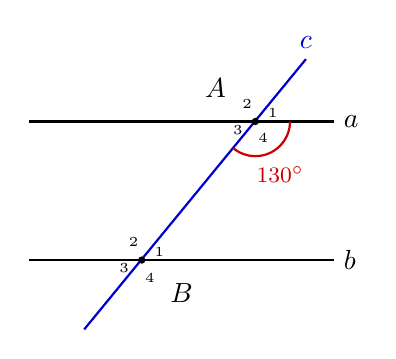
\begin{tikzpicture}[>=stealth, scale=0.88]
    \draw[thick] (-1.6, 2) -- (2.8, 2) node[right] {$a$};
    \draw[thick] (-1.6, 0) -- (2.8, 0) node[right] {$b$};
    \draw[thick, blue!80!black] (-0.8, -1.0) -- (2.4, 2.9) node[above] {$c$};
    
    \coordinate (A) at (1.67, 2);
    \coordinate (B) at (0.03, 0);
    
    \fill (A) circle (1.5pt);
    \fill (B) circle (1.5pt);
    
    \path (A) ++(140:0.75) node[font=\bfseries] {$A$};
    \path (B) ++(320:0.75) node[font=\bfseries] {$B$};
    
    \draw[red!80!black, thick] (A) ++(0:0.5) arc (0:-129.8:0.5);
    \path (A) ++(-65:0.85) node[red!80!black, font=\footnotesize] {$130^\circ$};
    
    \path (A) ++(25.1:0.28) node[font=\tiny] {$1$};
    \path (A) ++(115.1:0.28) node[font=\tiny] {$2$};
    \path (A) ++(205.1:0.28) node[font=\tiny] {$3$};
    \path (A) ++(295.1:0.26) node[font=\tiny] {$4$};
    
    \path (B) ++(25.1:0.28) node[font=\tiny] {$1$};
    \path (B) ++(115.1:0.28) node[font=\tiny] {$2$};
    \path (B) ++(205.1:0.28) node[font=\tiny] {$3$};
    \path (B) ++(295.1:0.28) node[font=\tiny] {$4$};
\end{tikzpicture}
\vspace{1.5mm}
&
\vspace{0.8mm}
\noindent\textit{Bài giải:}\par
\dongke{17}
\\ \hline
\end{tabularx}

\end{document}
